\documentclass[convert={density=400,size=640x480,outext=.png}]{standalone}
\usepackage{tikz}
\usetikzlibrary{calc}
\usepackage{hax}

\begin{document}
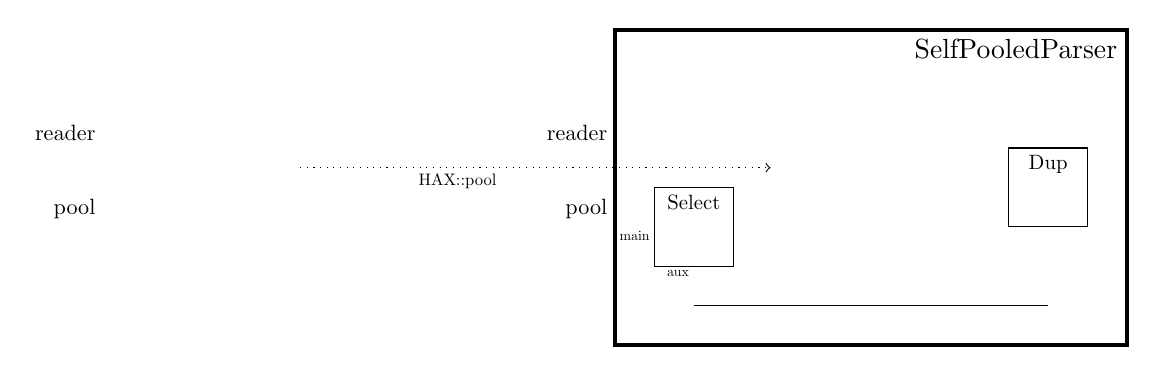
\begin{tikzpicture}[scale=0.5]
% lhs
\parser{(3,7)};
\node [above left, scale = 0.8] at (3,6) {reader};
\node [above left, scale = 0.8] at (3,4) {pool};
% mid
\draw [dotted,->] (8,5.5) -- (19.95,5.5);
\node [below, scale = 0.6] at (12,5.5) {HAX::pool};
% rhs
\parser{(20,7)};
\node [above left, scale = 0.8] at (16,6) {reader};
\node [above left, scale = 0.8] at (16,4) {pool};
\blockinput{(15,6)}{(20.5,6)};
% sel
\draw (17,3) rectangle (19,5);
\node [below, scale = 0.75] at (18,5) {Select};
\blockinput{(15,4)}{(17.5,4)};
\node [below left, scale = 0.5] at (17,4) {main};
\blockinput{(18,2)}{(18,3.5)};
\node [below left, scale = 0.5] at (18,3) {aux};
\blockoutput{(18.5,4)}{(20.5,4)};
% dup
\draw (26,4) rectangle (28,6);
\node [below, scale = 0.75] at (27,6) {Dup};
\blockinput{(25,5)}{(26.6,5)};
\blockoutput{(27.5,5)}{(30,5)};
\blockoutput{(27,4.5)}{(27,2)};
\draw (27,2) -- (18,2);
% outer
\draw [ultra thick] (16,1) rectangle (29,9);
\node [below left] at (29,9) {SelfPooledParser};

\end{tikzpicture}
\end{document}